\documentclass[12pt]{article}

\usepackage{graphicx}
\usepackage[margin=1.25in]{geometry}

\title{De Bruijn Graph Assembler}
\author{Kevin Boehme \and Shaun Miller \and Ken Reese}

\begin{document}
\maketitle

\section{Methodology}
Our error handling approach was quite simple. Once the reads were read in from the FASTA format and our algorithm broke them into the specified kmer length, we traversed the list of kmers looking for kmers that only appeared once. This effectively checked the support for each kmer in our list. If a kmer was found only once it would suggest a genotyping error and as such would be thrown out. If on the other hand, the kmer was supported multiple times, this suggests that it was correctly genotyped and was subsequently kept.  Our algorithm currently does not attempt to bridge non-branching nodes.

\section{Quality Analysis}
In order to analyze the quality of our assembly we relied on a few, informative metrics including average contig size, N50, number of contigs, and the maximum contig size. These metrics provided a solid foundation for determining the quality of our assembly (while adjusting kmer length) as well as providing a tractable means of comparing our assembly to other De Bruijn graph assemblers (such as Velvet).
Below are summary tables of our results for each of the synthetic datasets as well as the large and small, real datasets.

\begin{center}

\subsubsection*{Synthetic Dataset, Small Example, klen = 23}

\begin{tabular}{rl} \hline
Mean contig size: & 559 \\
N50: & 559 \\
Number of Contigs: & 1\\
Largest Contig Size: & 559\\
\label{table:synth_ex_small}
\end{tabular}

\subsubsection*{Synthetic Dataset, Small, klen = 18}

\begin{tabular}{rl} \hline
Mean contig size: & 63.5 \\
N50: & 99 \\
Number of Contigs: & 6\\
Largest Contig Size: & 142\\
\label{table:synth_small}
\end{tabular}

\subsubsection*{Synthetic Dataset, Large, klen = 21}

\begin{tabular}{rl} \hline
Mean contig size: & 163.3 \\
N50: & 459 \\
Number of Contigs: & 26\\
Largest Contig Size: & 1032\\
\label{table:synth_large}
\end{tabular}

\subsubsection*{Real Dataset, Small, klen = 42}

\begin{tabular}{rl} \hline
Mean contig size: & 382 \\
N50: & 1015 \\
Number of Contigs: & 3\\
Largest Contig Size: & 1015\\
\label{table:real_small}
\end{tabular}

\subsubsection*{Real Dataset, Large, klen = 57}

\begin{tabular}{rl} \hline
Mean contig size: & 149.5 \\
N50: &  232\\
Number of Contigs: & 251\\
Largest Contig Size: & 1558\\
\label{table:real_large}
\end{tabular}

\end{center}

We chose the given kmer lengths for the above assemblies from candidate lengths between 10 and 80.  The results shown above use an optimal\footnote{We here assumed that the optimal kmer length would be found between 10 and 80.} length as determined by a combined metric of the largest N50 value and largest contig produced by our assembler.

\section{Comparison}
We compared the results of our assembler with another De Bruijn graph assembler, Velvet. We used the large real dataset as our primary dataset for comparison because it was the most realistic one that both programs were optimized to assemble, and we felt it would have the most interesting results. The results of running the large real dataset for Velvet and our assembler are summarized in Tables and \ref{table:Velvet} \ref{table:kens} respectively. Our results appeared to be roughly comparable to the results Velvet achieved.

Velvet is only able to handle odd kmer lengths up to 31. Our algorithm however, has no kmer length limit and can handle both even and odd lengths. In this way our assembler implementation was more robust in terms of kmer length. It is also interesting to note that for kmer lengths 23 and 24, Velvets maximum length contig decreased dramatically (compared to the kmer lengths less 23 and greater than 24), but while still improving the N50 metric (See Table \ref{table:Velvet}). We did not observe a dip in max kmer length in our program (See Table \ref{table:kens}). Instead, we saw a continual improvement in assembly with increasing kmer size.

Since Velvet limits kmer sizes to 31 and below we couldn't compare the results of larger kmer lengths with Velvet. However, we do provide interesting plots demonstrating our assemblers continued improvement in assembly with kmer lengths greater than 31 (See figures \ref{fig:kmer_to_contig_large} , \ref{fig:kmer_to_contig_small} , \ref{fig:kmer_to_n50_large} , \ref{fig:kmer_to_n50_small}). Notice there comes a point where increasing kmer length significantly hurts the assembly, and this occurs with a shorter kmer length when the original contigs are shorter. Still, our algorithm was able to assemble longer contigs compared to Velvet using kmer lengths greater than 31.

\section{BLAST Results}
\subsection{Small Real Dataset}
This dataset maps to the sex determining region on the Y-chromosome, and encodes a testis-determining factor protein that initiates sexual differentiation.  Malfunctions in this gene are the cause of humans who are genetically male but developmentally female.

\subsection{Large Real Dataset}
Our largest contig matched Homo sapien chromosome 19- it’s part of the ABCA7 gene, of the ATP-binding cassette sub-family.  This gene is amazingly old and well-conserved across organisms---both prokaryotes and humans and most organisms in between have this gene conserved similarly in their genomes!

\section{Assembler Improvements}
Adding a method for bridging non-branching nodes would be an improvement.  We’d also like to add additional error handling--our method may not handle frame-shifts very well.  One specific method to do this is adding insertions and deletions to the k-mer creation algorithm.

\section{General Improvements for the Project}

\begin{enumerate}
\item It would be delightful to have more notice for this project- it’s great, but looking forward to and preparing for it from an earlier vantage point would have been really helpful! (We know we’re figuring some of this stuff out along the way, though.)

\item We also felt that using the online BLAST tools was much more interesting than the command line BLAST metrics we measured.  Getting a reasonably long contig and BLASTing it through the website yielded several graphical representations that were absolutely fascinating!  If part of the goal is to teach command line BLAST, that’s fine, but if command line BLAST is less important, just creating pretend reads off of real genetic data will allow us to BLAST against the NCBI database. And thanks for all of your hard work, folks, it’s a work in progress, but the trajectory this class is on is, in general, is a good one.

\end{enumerate}

\section{Group Contributions}
Ken's contributions included: use of his 4j solution (everyone contributed to addressing error handling), running the assembler to create the metrics, generation of plots/tables, and porting our google document into latex.

Kevin's contributions included: writing parts of this report (methodology, analysis, comparison, and this section), contributing to porting the google document to latex, setting up and running Velvet to get comparative metrics.

Shaun's contributions included: running BLAST on the generated contigs, writing parts of this report (BLAST, assembler improvements, and General Improvements), and editing all parts of this report.

We feel each member was able to contribute roughly equally to this project.

\begin{table}[p]
\centering
\begin{tabular}{|l|l|l|l|}
\hline
Kmer Size &Number of Contigs &N50 &Max Length\\\hline
10 &15122 &2 &36 \\
11 &7510 &10 &91 \\
12 &7510 &10 &91 \\
13 &2669 &31 &235 \\
14 &2669 &31 &235 \\
15 &1479 &63 &732 \\
16 &1479 &63 &732 \\
17 &1137 &76 &1112 \\
18 &1137 &76 &1112 \\
19 &1021 &84 &1275 \\
20 &1021 &84 &1275 \\
21 &872 &103 &1275 \\
22 &872 &103 &1275 \\
23 &776 &112 &884 \\
24 &776 &112 &884 \\
25 &645 &135 &1279 \\
26 &645 &135 &1279 \\
27 &521 &239 &1474 \\
28 &521 &239 &1474 \\
29 &456 &237 &1474 \\
30 &456 &237 &1474 \\
31 &347 &374 &1477\\\hline
\end{tabular}
\caption{Metrics for Velvet on Assembly of Large Dataset}
\label{table:Velvet}
\end{table}

\begin{table}[p]
\centering
\begin{tabular}{|l|l|l|l|} \hline
Kmer Size &Number of Contigs &N50 &Max Length\\\hline
10 & 7170 & 11 & 73 \\
11 & 3879 & 15 & 136 \\
12 & 2285 & 23 & 211 \\
13 & 1554 & 31 & 432 \\
14 & 1227 & 41 & 863 \\
15 & 1068 & 47 & 878 \\
16 & 962 & 54 & 1326 \\
17 & 898 & 61 & 1327 \\
18 & 835 & 71 & 1328 \\
19 & 789 & 82 & 1329 \\
20 & 739 & 93 & 1330 \\
21 & 682 & 103 & 1331 \\
22 & 645 & 111 & 1332 \\
23 & 637 & 111 & 1333 \\
24 & 619 & 114 & 1366 \\
25 & 592 & 115 & 1368 \\
26 & 568 & 119 & 1370 \\
27 & 525 & 144 & 1372 \\
28 & 504 & 148 & 1374 \\
29 & 483 & 166 & 1376 \\
30 & 455 & 177 & 1378 \\
31 & 424 & 190 & 1380 \\ \hline
\end{tabular}
\caption{Metrics for Our Assembler on Large Dataset}
\label{table:kens}
\end{table}

\begin{figure}[p]
\centering
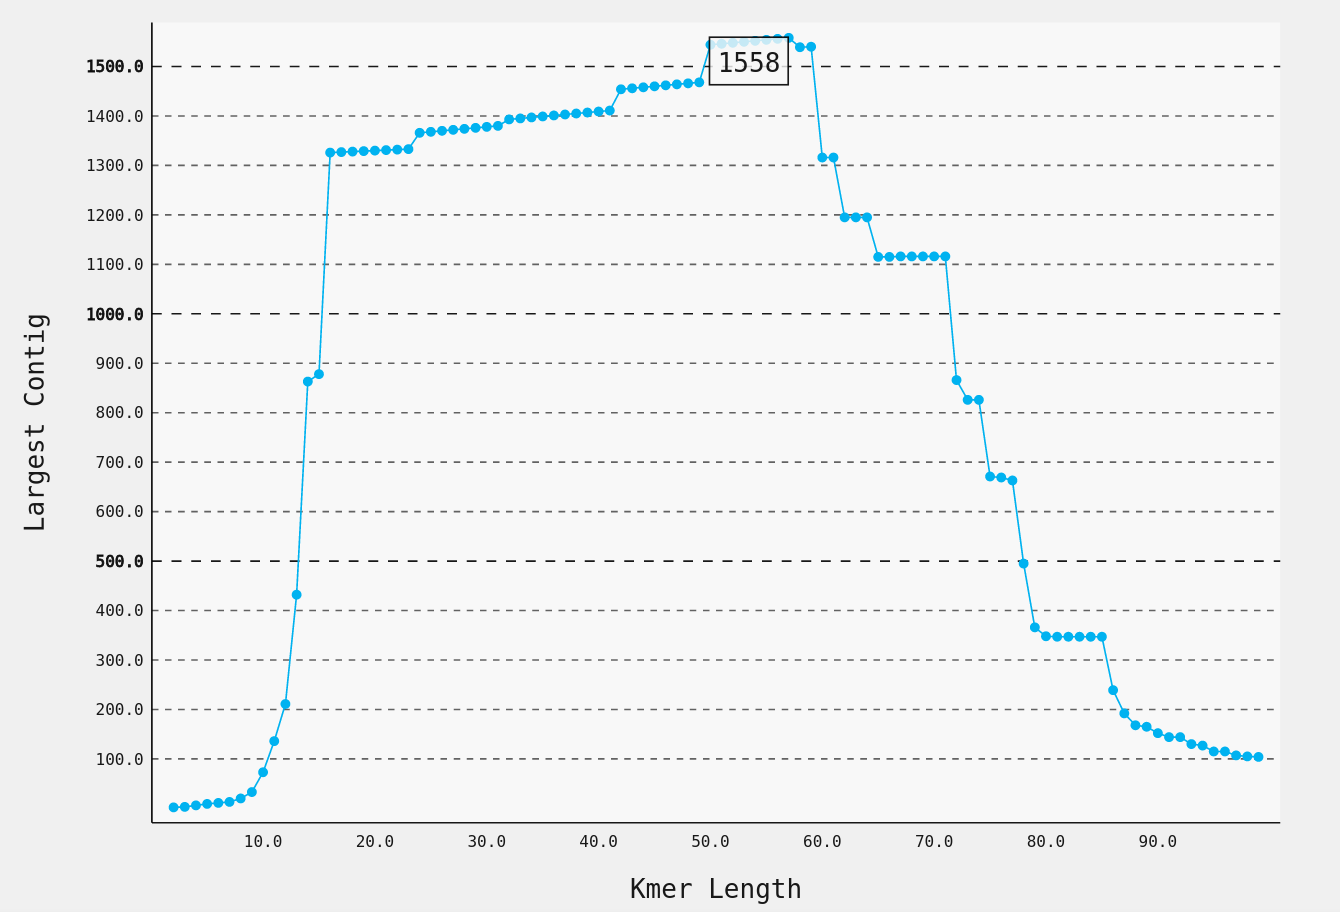
\includegraphics[width=5.25in]{klen_vs_largestcontig_large_fasta.png}
\caption{Kmer Length vs Longest Contig Size (Large Dataset)}
\label{fig:kmer_to_contig_large}
\end{figure}

\begin{figure}[p]
\centering
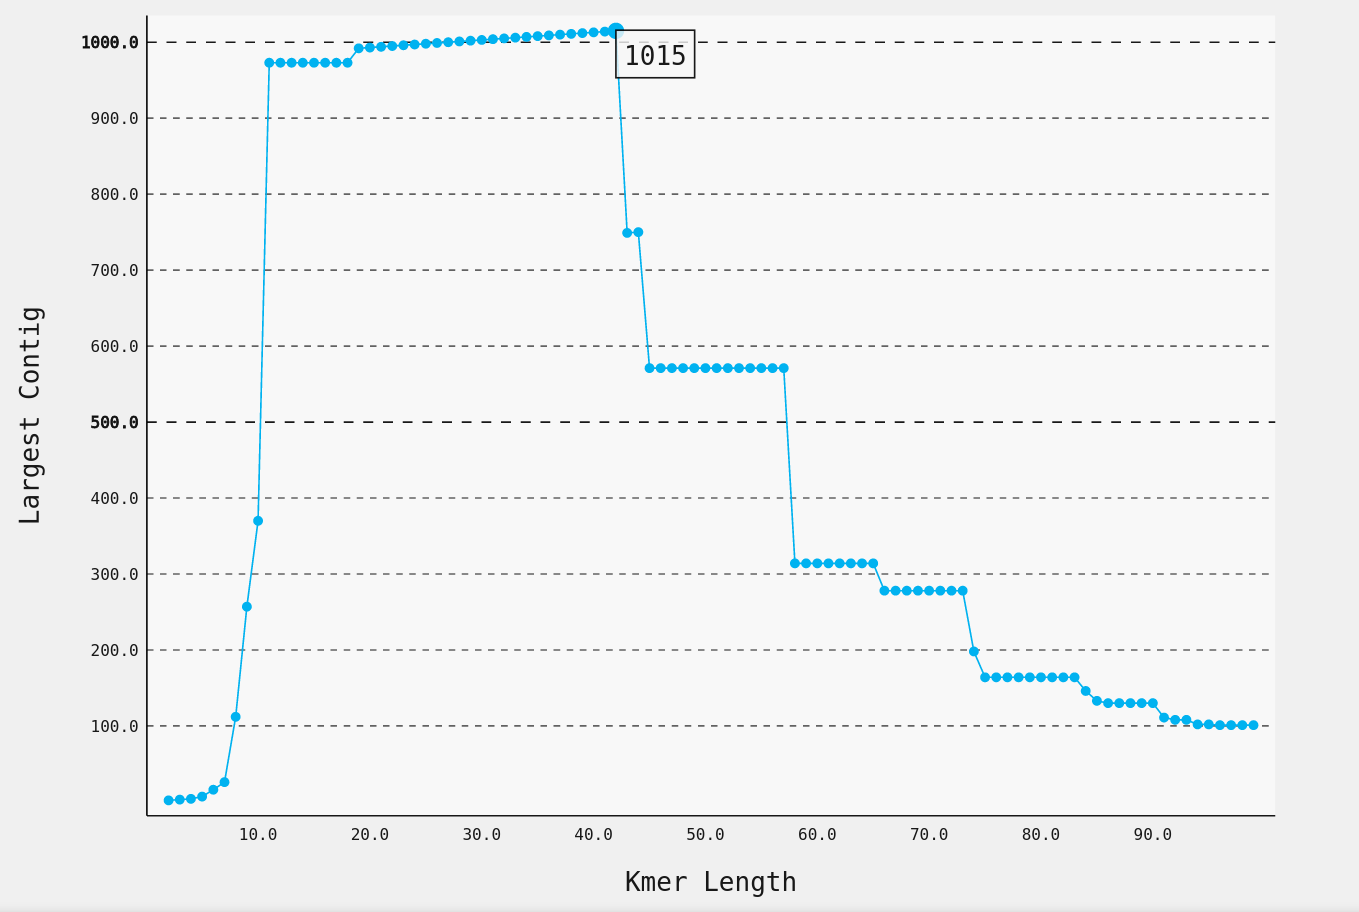
\includegraphics[width=5.25in]{klen_vs_largestcontig_small_fasta.png}
\caption{Kmer Length vs Longest Contig Size (Small Dataset)}
\label{fig:kmer_to_contig_small}
\end{figure}

\begin{figure}[p]
\centering
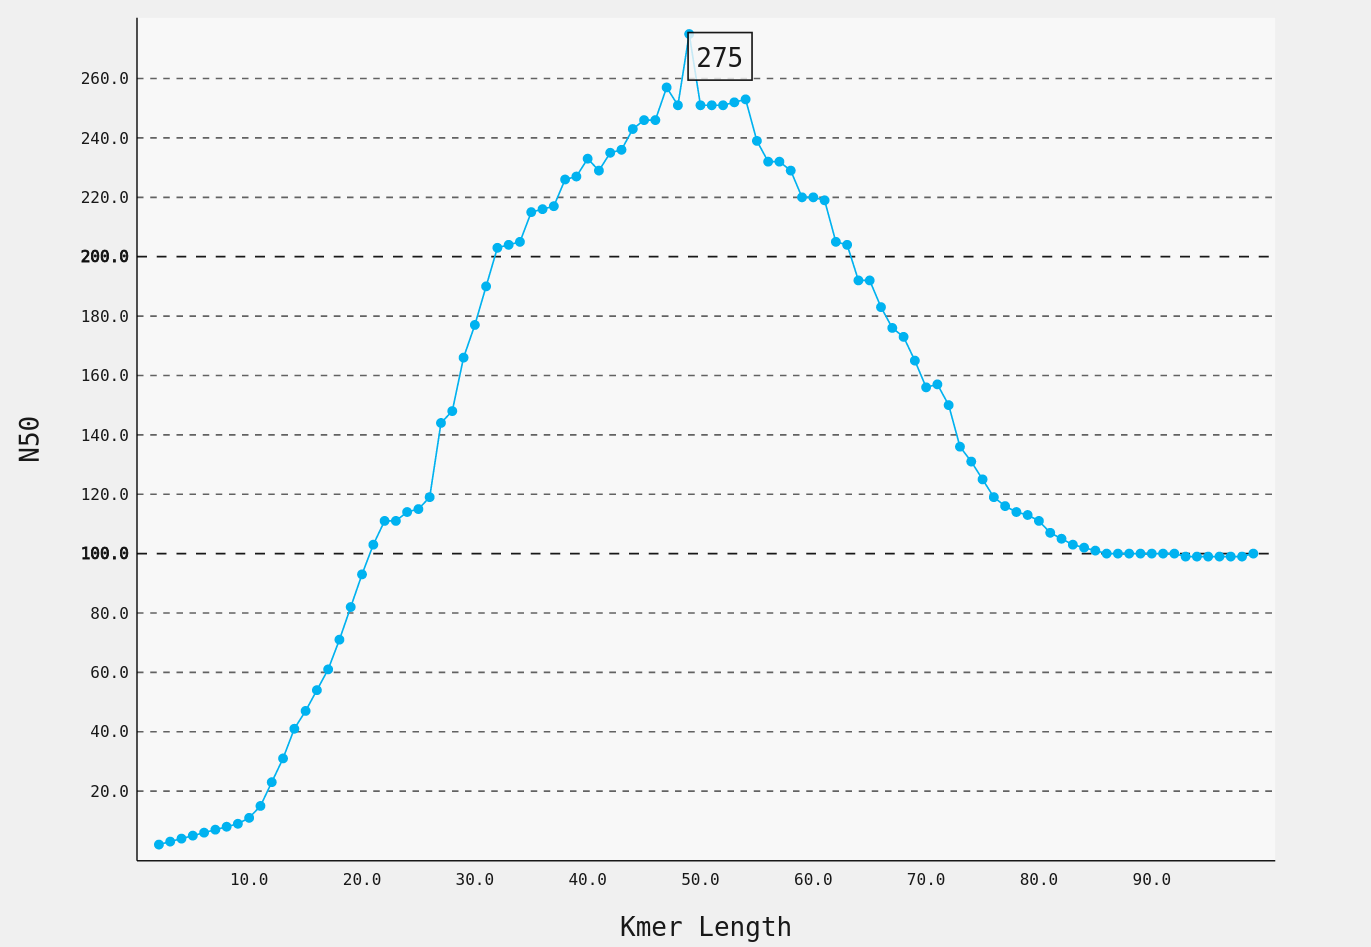
\includegraphics[width=5.25in]{klen_vs_n50_large_fasta.png}
\caption{Kmer Length vs N50 (Large Dataset)}
\label{fig:kmer_to_n50_large}
\end{figure}

\begin{figure}[p]
\centering
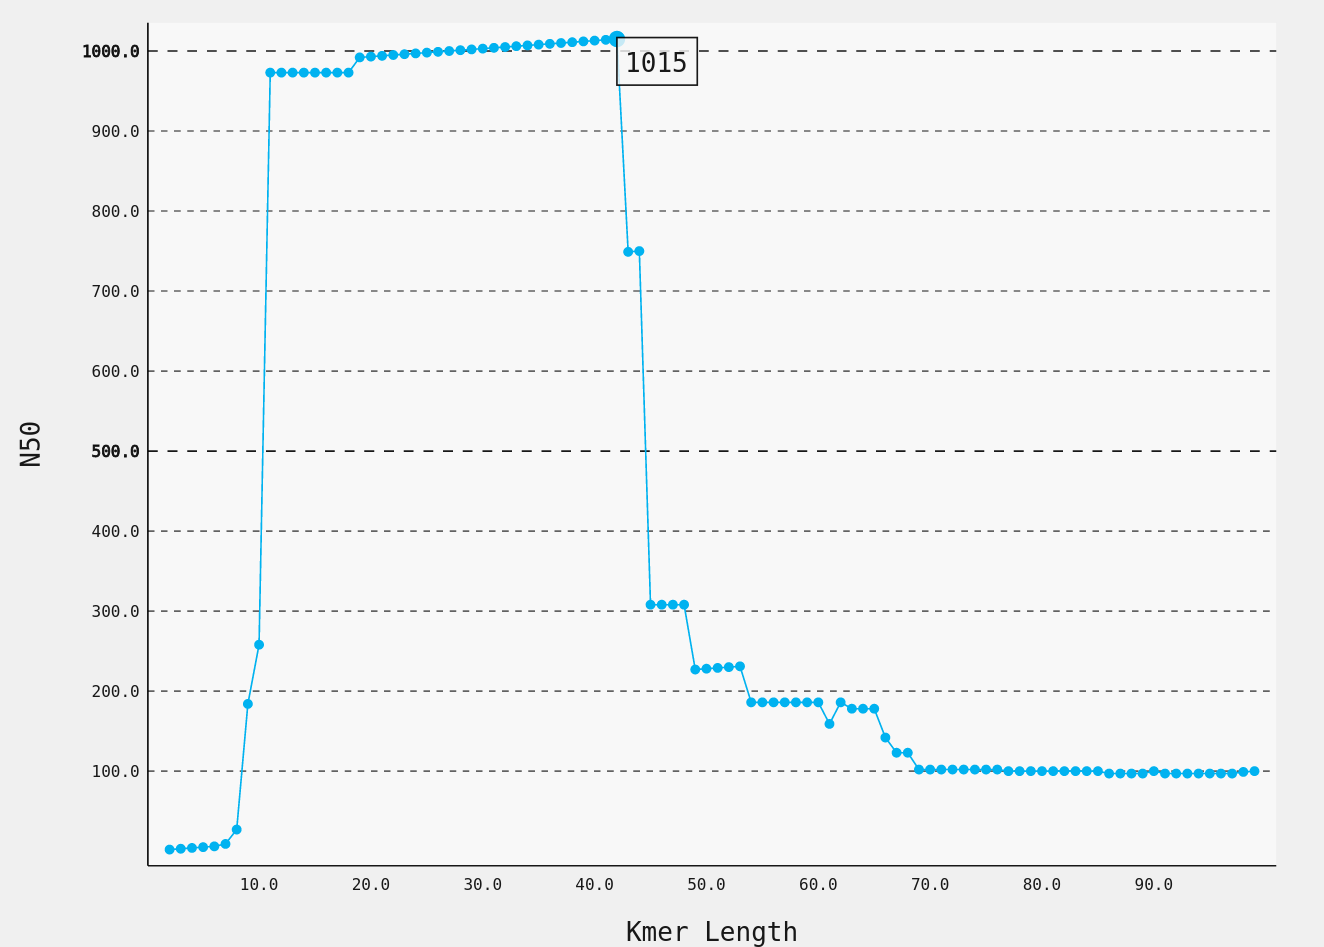
\includegraphics[width=5.25in]{klen_vs_n50_small_fasta.png}
\caption{Kmer Length vs N50 (Small Dataset)}
\label{fig:kmer_to_n50_small}
\end{figure}


\end{document}
